\chapter{Persistent Base Nodes}\label{chap:persistent-bases}

Updates begin their journey through the Soup data-flow graph at the base nodes,
after being successfully persisted to Soup's write-ahead log
(see~\ref{sec:soup-log}). While nodes further down in the graph might be
\textit{partial}, the base nodes always contain every single record a Soup
application has seen through its lifetime. This is crucial in maintaining a
balance between efficient read queries and space usage: popular queries will be
handled by partial state further down the graph, while reads for in-frequently
accessed rows will be able to refer all the way up to the source of truth, the
base nodes, through what in Soup is called a replay (see~\ref{sec:replays}). In
comparison to existing database systems, base nodes are closest to what
otherwise might be known as \textit{tables}.

\begin{figure}[H]
  \centering
  \includesvg[width=0.6\textwidth]{base-nodes}
  \caption{Updates enter the base nodes after being persisted to a write-ahead
  log.}
\end{figure}

While partial nodes can use \textit{eviction} (see~\ref{sec:eviction}) to keep
their memory footprint low, the size of base nodes will continue to grow
unbounded throughout a Soup instance's lifetime. In the short term this can be
handled by sharding Soup's data across multiple machines in a cluster, however
this is infeasible in the long term: sustained write workloads would continue to
grow the base node state, regardless of whether the data is accessed by queries
or not.

To combat this we would like to to move either parts of, or all of, the state
stored in base nodes to durable storage. This would reduce Soup's overall memory
usage, and perhaps even more significantly, transition Soup from a purely
in-memory database to a system that can store more data than its available
memory. With data safely persisted to base nodes, recovery after a failure would
also require less work, as partial nodes could gradually recover when data is
requested through replays. Summarized, introducing persistence to Soup's base
nodes would achieve the following goals:

\begin{enumerate}
  \item Prevent Soup's memory usage from growing unbounded over time
  \item Support larger-than-memory data sets
  \item Reduce recovery time after failures
\end{enumerate}

\section{In-Memory State}\label{sec:in-memory-state}
The current in-memory state implementation provides a key-value API with support
for multiple indices. A separate state data structure is kept for each
materialized node, including base nodes. The same data structure is used by both
partially and fully materialized nodes, however as base nodes always have to be
fully materialized this section will omit describing details regarding the
former. The state data structure will be referred to as \code{State}.

\subsection{Adding indices}
The \code{State::add\_key} method introduces a new index to a specific \code{State} map,
and takes a set of columns as its argument. Additional indices do not lead to
multiple copies of the data, but rather contain pointers to the existing rows.
These pointers are held in separate data structures however: each new index
introduces a new hash map structure responsible for answering queries for that
specific set of columns.

New indices have to be \textbf{built}, as they are expected to answer queries
for data that has already been inserted, right away.

\begin{listing}[H]
  \begin{minted}[frame=lines]{rust}
state = State()
// Initialize `state` with an index on the first column:
state.add_key([0])

// Then insert two rows:
state.insert([A, 1])
state.insert([B, 1])
assert_equal(state.lookup(A), [[A, 1]])

// Now, add an index on the second column:
state.add_key([1])
// ...which should return values that existed prior to the index being added:
assert_equal(state.lookup(1), [[A, 1], [B, 1]])
  \end{minted}

  \caption{Pseudo-code test that shows the expected behavior for adding indices
  with existing values.}\label{lst:existing-index}
\end{listing}

\subsection{Retrieving rows}
A stateful map would not be useful without a method for retrieving data, which
\code{State} provides through \code{State::lookup}. This takes a set of columns
and a key as its arguments, and make use of a \textbf{single} index to retrieve
one or more existing values. Each index is held in a separate hash map, and
retrievals can thus be completed in constant time.

That \code{State::lookup} can return more than one value is an important
distinction from most key-value stores, and is absolutely crucial in
implementing secondary indices. Without it \code{State} would only be able to
serve as an index structure for \textit{unique primary keys}.

\subsection{Inserting rows}
Naturally, to be able to read anything in the first place, we first need to
insert data into our stateful data structure. This is done through the
\code{State::insert} method, which takes a single row as its argument.
\code{State::insert} is responsible for updating every index in \code{State},
and has to loop through and insert a pointer for each included index.

\subsection{Removing rows}
Similar to insertions, removals have to update all indices. Contrary to what one
might expect, \code{State::remove} takes a single row as argument, and not a
key. This is due to how \code{State} is used in Soup: as an internal storage
unit for partially and fully materialized nodes alike. While it might make sense
for a base node to only delete rows by key, other nodes might need support for
deleting a single row, regardless of if its key is unique or not. No matter,
translating \code{remove(row)} to \code{remove(key)} is trivial, as shown in
listing~\ref{lst:removals}.

\begin{listing}[H]
  \begin{minted}[frame=lines]{rust}
state = State()
state.add_key([0])
state.insert([A, 1])

row = state.lookup(A)
state.remove(row)
  \end{minted}

  \caption{Deleting a row from a base node in Soup.}\label{lst:removals}
\end{listing}

\subsection{Updating rows}
Similar to how \code{State} does not have a method for removing by key,
\code{State} does not include a method for updating a single row. Updates are
instead handled by the base node's logic, by first emitting a negative
record---to delete the existing row---followed by a positive one to insert the
new value.

\section{Requirements}\label{sec:requirements}
Random access memory is, and has been for years now, fast. Durable storage is
undergoing a similar transformation with the recent introduction of NVMe
SSDs~\cite{nvme}, but is still orders of magnitudes slower than RAM.\@ This
means that while introducing persistent storage into parts of the Soup equation
comes with many benefits, increased performance is not likely to be one of them.
Rather, the goal will be to maintain the existing performance characteristics,
while still achieving our three main goals.

\subsection{Write throughput}
Backfills of missing state, replays, go through the regular update paths in the
Soup data-flow graph. An increase in processing latency at the base nodes would
not only reduce the write throughput, but also have a significant impact on
reads that require a replay to complete.

\subsection{Point query performance}
Base node queries should be a seldom occurrence, as most queries should be
served by nodes further down the graph. Still, when a query eventually makes it
all the way up to the base nodes, it is important that it can be completed fast
enough to not significantly slow down the total read throughput of the system.
Slightly higher latency is on the other hand to be expected, we are after all
comparing persistent storage to an in-memory hash map.

\subsection{Support both primary and secondary indices}
Similar to Soup's existing \code{State} implementation, a durable replacement
has to support mapping a single key to multiple values, \ie secondary indices.

\section{Embedding an existing storage engine}
On-disk data structures have wildly varying performance characteristics. A
B+tree (see~\ref{sec:btree}) might perform well on random reads, but get heavily
out-performed by an LSM-tree (see~\ref{sec:rocksdb}) on sequential writes. At
the same time, decades of changes in hardware research have broadened the field
even further. A new NVMe SSD is able to reach almost half a million random reads
per
second\footnote{\url{http://www.samsung.com/semiconductor/minisite/ssd/product/consumer/ssd960/}},
whereas a traditional spinning disk barely scratches the surface of a
hundred\footnote{\url{https://www.symantec.com/connect/articles/getting-hang-iops-v13}}.
This makes building data structures for durable storage non-trivial and time
consuming.

On the other hand, there is a plethora of existing, open-source, storage
backends available today. Similar to their underlying data structures, different
backends are built for different use cases, with different hardware in mind.
This provides an option to implementing data structures from scratch, by instead
making use of existing database systems to test performance assumptions, which
is exactly what this thesis will do: first using SQLite, and later using
RocksDB.\@

\subsection{State Interface}\label{sec:trait}
Before diving into the individual \code{State} operations, we need to pave the
way for the possibility of even having two different state implementations: the
existing in-memory implementation, and the new persistent storage variant, from
here on referred to as \code{MemoryState} and \code{PersistentState}. This is
achieved by turning the existing \code{State} implementation into an
interface---a \textit{trait} in Rust---which would then be implemented by both
the \code{State} variants. This helps maintain the current status quo where
\code{State} is an \textit{abstract data type}: internal Soup callers do not
need to be aware of the location their data is getting stored---they can simply
interact with the \code{State} trait as a black box\@.

\begin{listing}[H]
  \begin{minted}[frame=lines]{rust}
pub trait State {
    /// Add an index keyed by the given columns.
    fn add_key(&mut self, columns: &[usize]);

    /// Inserts or removes each record into State
    fn process_records(&mut self, records: &Records);

    /// Retrieve values from the index defined for `columns`.
    fn lookup<'a>(
      &'a self,
      columns: &[usize],
      key: &KeyType
    ) -> LookupResult<'a>;

    /// Count the rows currently stored in `State`.
    fn rows(&self) -> usize;

    /// Return a copy of all records.
    fn cloned_records(&self) -> Vec<Vec<DataType>>;
}
  \end{minted}

  \caption{\
    A segment of the main methods defined in our \code{State} trait.
  }\label{lst:state}
\end{listing}

As code is often more succinct than prose, a subset of the \code{State} trait is
shown in listing~\ref{lst:state}. The rest of the methods have been omitted for
clarity, as they are only relevant to nodes that can be partially
materialized---not base nodes. Similarly, some of the methods take in extra
arguments related to partial state---omitted here.

Comparing the trait in listing~\ref{lst:state} to the operations described
in~\ref{sec:in-memory-state} you might notice that the insert and removal
operations are gone. These have been abstracted into a higher level method:
\code{process\_records}. Every packet in Soup has the potential to contain more
than one record by being a merged packet, due to \textit{group commit}
(see~\ref{sec:group-commit}). Because of this, the function responsible for
materializing records in a node's \code{State} would go through a packet's
records, individually calling methods like \code{State::insert} and
\code{State::remove}. This is completely valid for an in-memory implementation,
where each operation has the same cost---without any initial overhead. This is
not the case for writes to potentially slower, durable storage. Here batching is
key, and an indicator to the underlying methods that they can perform operations
in one go is crucial.

\subsection{Retrieving rows from \code{State}}
While other languages might implement memory safety through garbage collection
or manual memory management, Rust does the same through ownership, as described
in~\ref{sec:rust}. Whenever a value goes out of scope, it is deallocated. How
do you know when a value goes out of scope? In a garbage collected system, this
happens when there are no longer any references to the value. In Rust, each
value only has one owner, and any references need to live \textbf{at least} as
long as the value created by that owner.

However, what if a value needs to be owned by more than one location? That is
often the case for data structures, and \code{State} is no exception here.
Values stored in \code{MemoryState} should not have to be cloned during
retrieval, which would incur a heavy performance penalty. Instead, retrieving
values from \code{State} return dynamically reference
counted\footnote{\url{https://doc.rust-lang.org/std/rc/index.html}} values,
allowing shared ownership of a single value by counting owners at runtime.
Subsequent retrievals of the same value always point to the same memory
location, with the source of truth being stored in \code{State}.

\todo{add a figure showing the difference between retrieving rows from memory
and from durable storage}

What if, on the other hand, a row does not exist in memory to begin with? This
would be the case when data is retrieved from durable storage: after reading a
row in its on-disk representation and de-serializing it to a value in Soup's
data format, where is that very value stored? The \textit{data} used to create
the value exists on disk, but the actual memory representation of the value was
just created. While \code{MemoryState::lookup} would want to return a reference
to an internally stored value, \code{PersistentState::lookup} would rather want
to hand over ownership of the value to the caller. Enter the
\code{Cow}\footnote{\url{https://doc.rust-lang.org/std/borrow/enum.Cow.html}}
---a \textbf{clone-on-write} pointer from Rust's standard library that helps
with this exact purpose, by allowing data to be represented either as
\code{Borrowed} in the case of \code{MemoryState} or \code{Owned} for
\code{PersistentState}.

Additionally, the rows returned from \code{State::lookup} are wrapped in a
\code{LookupResult} enum, representing either a found or a missing value. The
latter is never relevant for \code{PersistentState}, which is only used to
represent fully materialized state. Note that a \textit{miss} does not signify
that the value does not exist, it simply means that this particular \code{State}
does not have it, while a \code{State} instance further up the data-flow graph
does.

\begin{listing}[H]
  \begin{minted}[frame=lines]{rust}
// Before:
pub enum LookupResult<'a> {
    Some(&'a [Rc<Vec<DataType>>]),
    Missing,
}

// After:
pub enum RecordResult<'a> {
    Borrowed(&'a [Rc<Vec<DataType>>]),
    Owned(Vec<Vec<DataType>>),
}

pub enum LookupResult<'a> {
    Some(RecordResult<'a>),
    Missing,
}
  \end{minted}
  \caption{\
    Prior to the introduction of \code{PersistentState}, reads from \code{State}
    would always result in a borrowed, reference counted value. Now that only
    happens for reads from \code{MemoryState}---with \code{PersistentState} the
    caller is responsible for retaining ownership of the value.
  }\label{lst:existing-index}
\end{listing}

\subsubsection{Using \code{LookupResult}}
Introducing the potential of a returned row being either \code{Borrowed} or
\code{Owned} has its downsides. For one, callers would have to handle both
branches, as the \textit{type} contained in a borrowed value is different from
the \textit{type} in an owned one. In the former, callers would always have to
clone the value to hand it over to someone else, whereas in the latter, they
could simply \textit{move} it out. The difference here comes from the
expectations of the value: a borrowed value implies that someone wants to retain
ownership of it---\eg it has to be cloned to give ownership to someone
else---while an owned value is the responsibility of the caller.

\begin{listing}[H]
  \begin{minted}[frame=lines]{rust}
if rows.len() > 0 {
  match rows {
    RecordResult::Owned(mut rows) => {
      out.push(Record::Negative(rows.swap_remove(0)))
    }
    RecordResult::Borrowed(rows) => {
      out.push(Record::Negative((*rows[0]).clone()))
    }
  }
}
  \end{minted}
  \caption{\
    With \code{RecordResult}, returned values can be either \code{Borrowed} or
    \code{Owned}, making callers responsible for handling both use cases. Here
    a negative record---used to signal to descendant nodes that this value
    should be invalidated---is emitted using the first row as its value.
  }\label{lst:cow}
\end{listing}

As is often the case, this can be simplified by looking at what the callers are
actually using the returned values for. The unpacked \code{rows} variable in
listing~\ref{lst:cow} is---as the name implies---a list of rows. Taking this
collection, and \textit{iterating} over either all of, or a subset of, the rows,
before returning a new iterator over the potentially modified values, was by far
the most common operation. Instead of delegating the responsibility for doing so
to the callers, this can be implemented on \code{RecordResult} itself, greatly
simplifying use cases like listing~\ref{lst:cow}.

\begin{listing}[H]
  \begin{minted}[frame=lines]{rust}
if let Some(row) = rows.into_iter().next() {
    out.push(Record::Negative(row.into_owned()));
}
  \end{minted}
  \caption{\
    The option of turning a \code{RecordResult} into an iterator is used to
    simplify the logic from listing~\ref{lst:cow}.
  }\label{lst:cow-better}
\end{listing}

\todo{write about IntoIterator and how it yields cows.} \\
\todo{include a more formal specification of how this works?}

\section{Persistent State with SQLite}
The first iteration towards a durable state implementation uses SQLite as its
storage engine. Described in section~\ref{sec:sqlite}, SQLite is a well-tested,
heavily used system with a track record in everything from applications to other
databases. SQLite uses B+trees internally---a reasonable, no frills data
structure with easy-to-reason about performance guarantees. This makes it useful
for a first prototype, and will help us answering the question of whether a
B+tree based \code{PersistentState} is feasible following the requirements
defined in~\ref{sec:requirements}. We will use the Rusqlite~\cite{rusqlite}
library for calling into SQLite from Rust.

\subsection{Schema}

SQLite is an embedded database, and requires no inter-process communication to
function. When persisting data, SQLite writes directly to durable files. This
requires exclusive locks to be held while writing (see~\ref{sec:sqlite-locks}),
eliminating the possibility of simultaneous updates from parallel locations to
the same database. This is not an issue for Soup and \code{PersistentState}.
Soup's \code{State} instances are completely standalone, and each
\code{PersistentState} instance can operate against a separate SQLite database,
avoiding the need for locks altogether.

SQLite---like SQL databases in general---require a strict schema to be defined
at all times. How this schema looks is usually a result of what kind of queries
a database needs to respond to, which in Soup's case depends on the indices a
specific \code{State} instance has been given responsibility for. Each column in
a Soup index will be given a column in the SQLite table, allowing flexible read
queries on any of the given indices. The row itself will be stored in a separate
column, serialized using \code{bincode} (see~\ref{sec:bincode}).

\subsection{Adding indices}

Each call to \code{State::add\_key} sets up that specific \code{State} instance
for queries on the given set of columns. This primarily involves extending our
SQLite schema with the newly given columns, while creating an actual SQLite
index on the \textit{column combination} itself. The latter is not strictly
necessary: SQLite is able to retrieve data for any columns, regardless of
existing indices. The performance would be exceedingly poor however, as it would
require scanning the entire table.

As an example, consider a Soup base node with the three columns \code{(a, b,
c)}. Queries further down the graph dictate that the base node needs to be able
to efficiently read rows by the columns \code{(a, b)}, and by only \code{c}.
After a series of inserts, our SQLite table for the base node's
\code{PersistentState} might look something like table~\ref{table:sqlite}.

\begin{table}[H]
  \centering
  \begin{tabular}{l l l l}
    \toprule
    \textbf{\code{a}} & \textbf{\code{b}} & \textbf{\code{c}} & \textbf{\code{row}} \\ \midrule
    1 & cat & norway & \code{bincode(1, cat, norway)}   \\ \midrule
    2 & dog & sweden & \code{bincode(2, dog, sweden)}   \\ \midrule
    3 & fish & denmark & \code{bincode(3, fish, denmark)} \\ \bottomrule
  \end{tabular}

  \caption{\
    An underlying SQLite table in \code{PersistentStore} after a few inserts.
    \code{bincode()} is used to signify that the value is serialized in the
    bincode binary serialization format.
  }\label{table:sqlite}
\end{table}

\subsection{Retrieving rows}

After the hard work of building the indices has completed, a myriad of rows is
only a \code{SELECT}-statement away. \code{PersistentState::lookup} takes a set
of columns and values for those columns as arguments, which are then translated
a \code{SELECT}-query. Considering the example in our previous section, the key
\code{(1, cat)} for the columns \code{(a, b)} would result in a query on the
form of \code{SELECT row FROM store WHERE index\_0 = 1 AND index\_1 = "cat"},
which SQLite can then complete in a timely manner due to the index on \code{(a,
b)}.

\subsection{Inserting rows}

Given a vector of values, \code{PersistentState} has to first extract the
columns necessary for its current set of indices and so that their values can be
translated to SQLite friendly types. These can then be used to build an
\code{INSERT}-query on the form of \code{INSERT INTO store (index\_0, index\_1,
row) VALUES (\ldots)}, where \code{row} is a binary representation of the entire
vector, serialized using \code{bincode}.

\subsection{Removing rows}

Similar to lookups, removals need to first build a \code{WHERE}-clause by
extracting the index column values from the target row, which can then be used
to perform a \code{DELETE}-statement on the form of \code{DELETE FROM store
WHERE index\_0 = 1 AND index\_1 = "cat"}.

\subsection{Processing insertions and removals}

All mutations need to be done within a transaction in SQLite, and operations
performed without an explicit transactions are implicitly given one. Performing
a single transaction is potentially expensive in SQLite, especially with strong
durability guarantees, where each transaction will incur a \code{fsync}
operation to make sure updates are successfully persisted before returning.

Instead, \code{PersistentState} batches all mutations required for a single
packet (per base node) into one transaction. This is done using the
\code{State::process\_records} method described in~\ref{sec:trait}, as shown in
listing~\ref{sec:process-sqlite}.

\begin{listing}[H]
  \begin{minted}[frame=lines]{rust}
fn process_records(&mut self, records: &Records) {
    let transaction = self.connection.transaction().unwrap();
    for r in records.iter() {
        match *r {
            Record::Positive(ref r) => {
                Self::insert(r.clone(), &self.indices, &transaction);
            }
            Record::Negative(ref r) => {
                Self::remove(r, &self.indices, &transaction);
            }
        }
    }

    transaction.commit().unwrap();
}
  \end{minted}

  \caption{Multiple insertions and removals are wrapped in a transaction.}\label{lst:process-sqlite}
\end{listing}


\subsection{Counting rows}

An accurate count of the total rows in the database can be retrieved using an
SQL \code{COUNT}-query: \code{SELECT COUNT(row) FROM store}.

\subsection{Replacing the Soup write-ahead log}

Soup already writes all updates to durable storage in the form of a write-ahead
log. After an unexpected failure, Soup replays entries in the log to recover its
state to what it was prior to crashing. This is far from optimal for long
running applications (which most databases are), where recovery time would
simply continue to grow unbounded. Relying on SQLite for durability would let
Soup recover directly from SQLite's database files---a much faster operation
than replaying the entire log.

Modern SQLite versions make use of a write-ahead log to ensure durability
(see~\ref{sec:sqlite-wal}) while maintaining high write performance. Relying on
SQLite's WAL instead of Soup's requires some refactoring however: up until now
Soup has sent out acknowledgments of writes as soon as the write is merged into
a batch by the group commit protocol, prior to inserting the packet itself into
Soup's data flow graph. Materialization into \code{PersistentState} happens
after this on the other hand, while the packet is being processed by a base
node. This comes with a minor write latency penalty regardless of the
\code{State} implementation, as more work needs to happen before an
acknowledgment can be sent.

\begin{figure}[H]
  \centering
  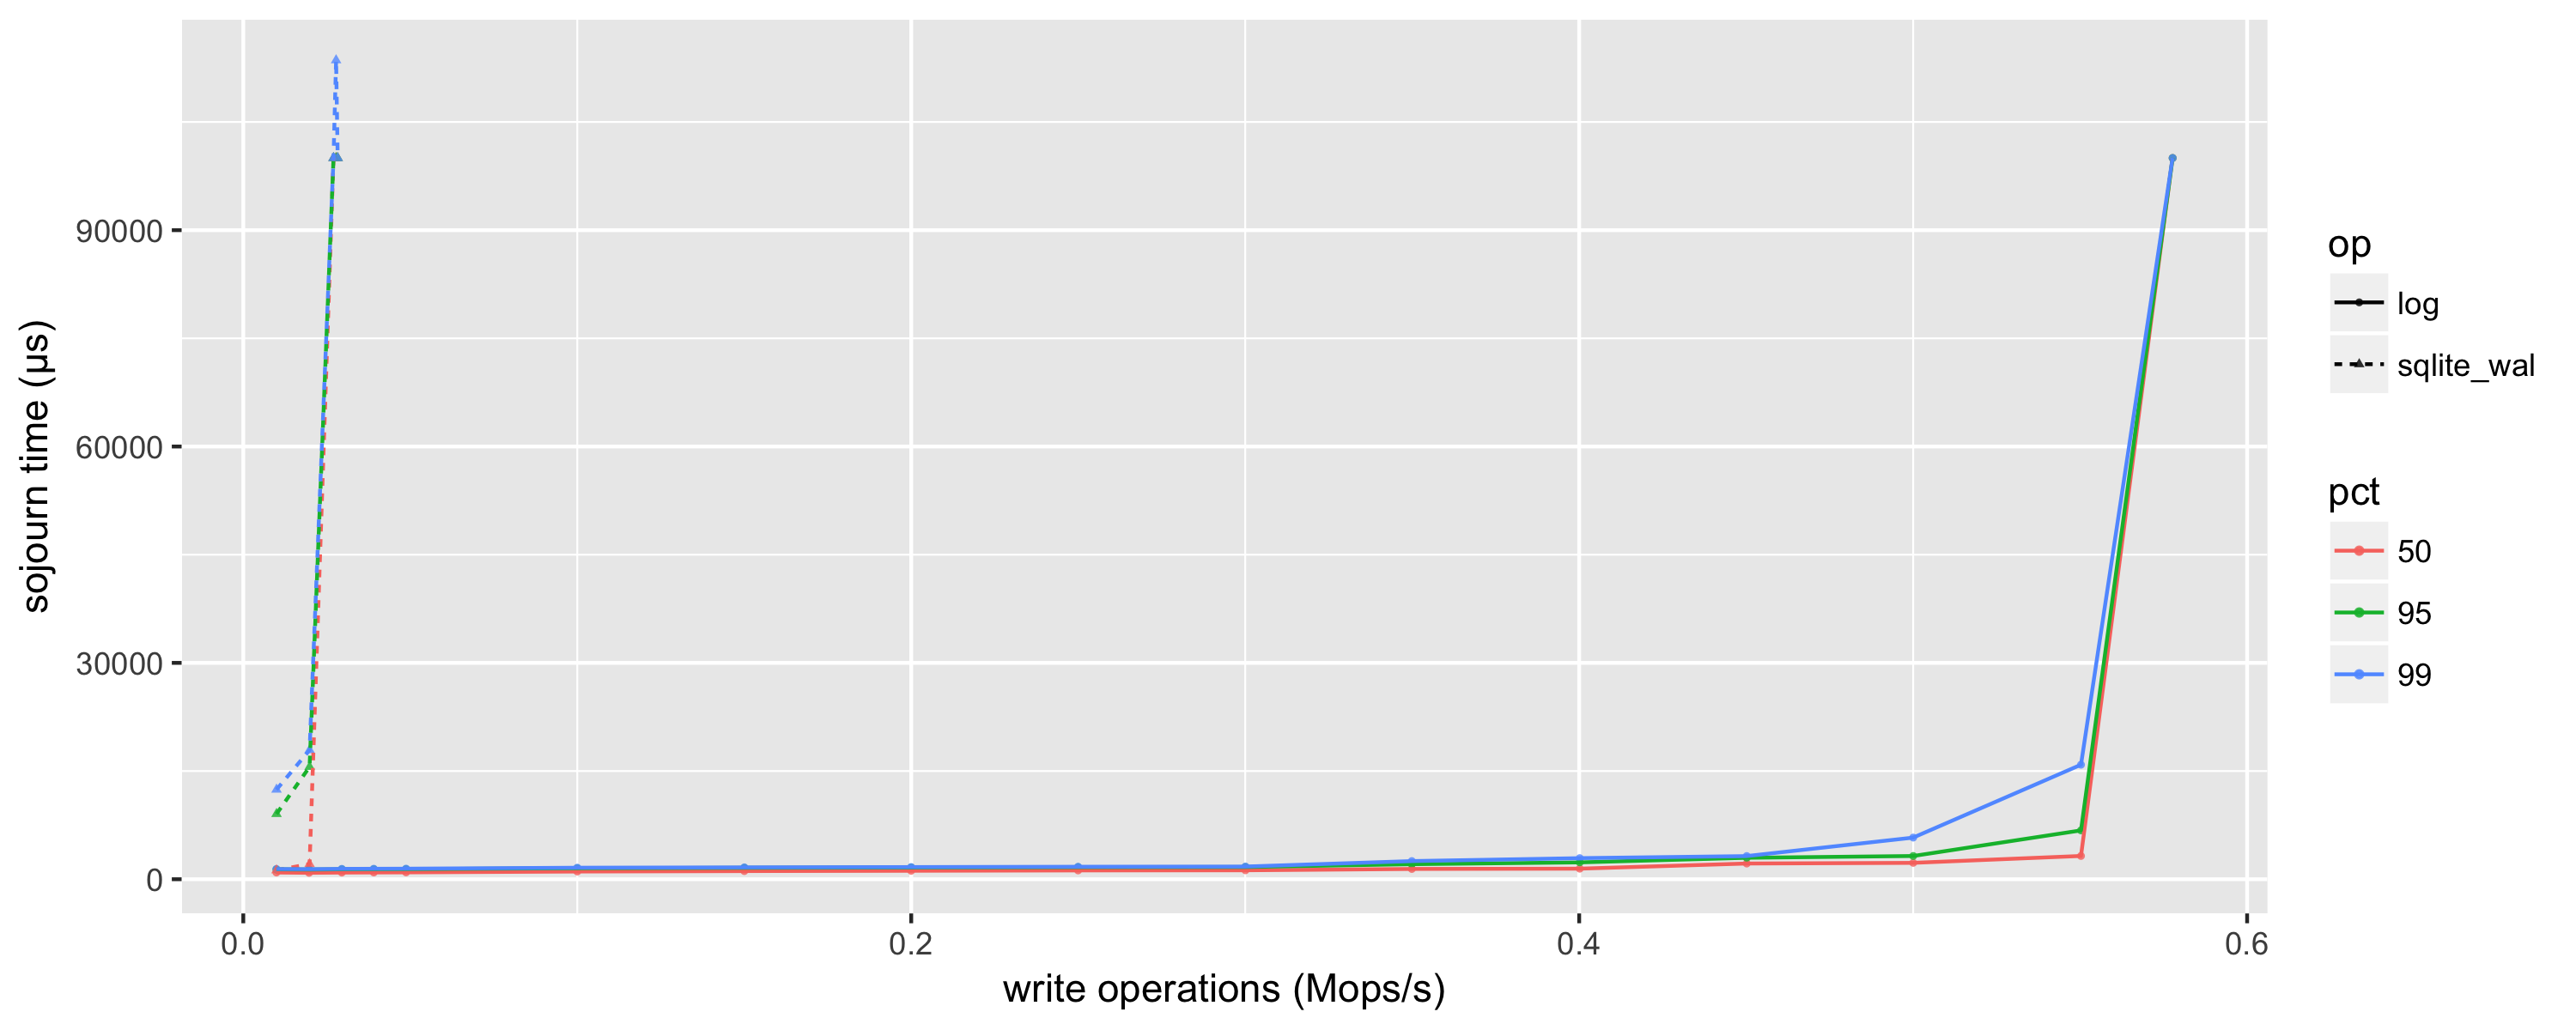
\includegraphics[width=\textwidth]{graphs/sqlite-wal-sjrn}
  \caption{\
    Write-only throughput measured using the \code{vote} benchmark. \code{log}
    relies on Soup's WAL for durability and stores base node state in-memory.
    \code{sqlite\_wal} uses SQLite for durability, storing all base node state
    on persistent storage.
  }\label{graph:sqlite-wal}
\end{figure}

Intuitively, one might expect writes to SQLite to be at least somewhat slower
than writes to Soup's regular write-ahead log, simply from the fact that the
latter needs to write less data to disk. At the same time, the WAL
implementation in SQLite is surely far more sophisticated than Soup's. SQLite's
WAL consists of a series of frames, allocated ahead of time to avoid unnecessary
resizing at every insertion. Soup's WAL is on the other hand purely an
ever-growing sequential file, where entries are appended to the end of the file
for each new packet. So why---as shown in figure~\ref{graph:sqlite-wal}---is
SQLite so much slower?

\subsubsection{Checkpointing}

With an arsenal of profiling tools at our disposal, guessing is unnecessary. A
flame graph built from profiling data recorded with \code{perf} quickly
highlights the two main culprits: checkpoints and B-tree updates. As mentioned
in section~\ref{sec:sqlite-checkpoints}, SQLite automatically transfers data
from the WAL to its main database file once the WAL exceeds a certain threshold.
Checkpointing---similar to everything else in SQLite---is a synchronous
operation, incurring a significant latency penalty once it happens. Regardless,
checkpointing is a necessary evil. Up until the point of a checkpoint, reads
have to refer to both the content in the WAL and the content in the main
database. Delaying the automatic checkpoint operation does not make much of a
difference either, as it results in more content to copy over when the
checkpoint finally occurs.

\begin{figure}[H]
  \centering
  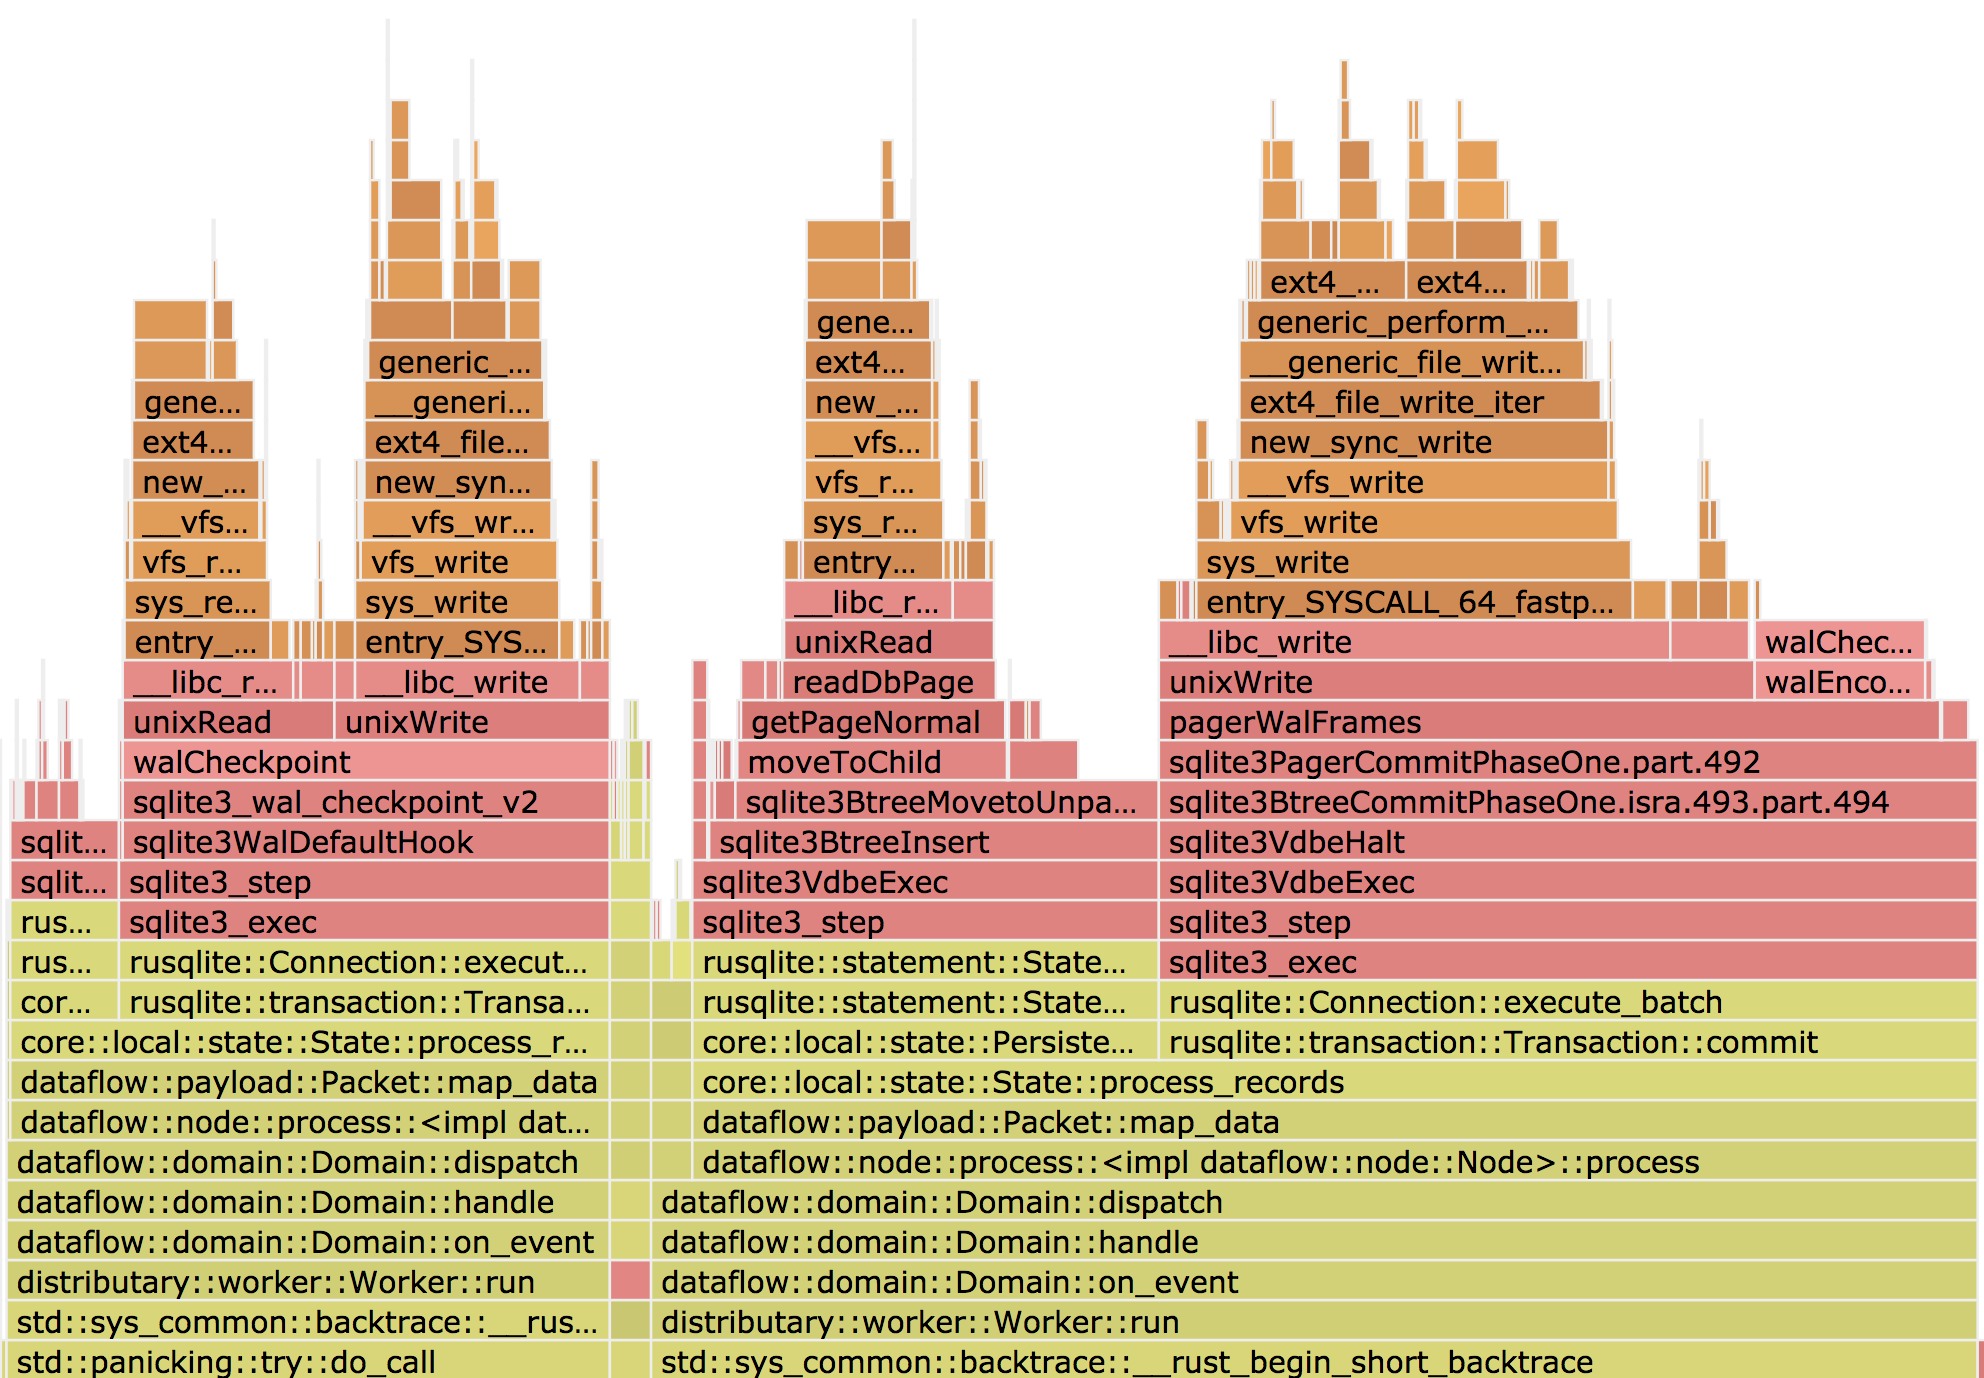
\includegraphics[width=\textwidth]{sqlite-wal-flame}
  \caption{A flame graph highlighting time consuming functions in
  \code{PersistentState}.}\label{fig:sqlite-wal}
\end{figure}

Does checkpoints have to happen synchronously, before a write acknowledgment is
sent to a client? In reality, they do not: taking a checkpoint does not make any
difference in terms of durability. Instead, \code{PersistentState} can issue a
checkpoint manually after a certain amount of time, but \textit{after}
acknowledging any outstanding writes. This had a minor effect on throughput,
taking it from a measly 27k ops/s, to at least 42k ops/s---still far too slow.
The checkpoints still happen synchronously, pausing processing at that specific
\code{PersistentState} instance for a significant amount of time instance for a
significant amount of time.

That leads to the question of whether checkpoints have to happen in the same
thread as regular processing altogether. The SQLite manual mentions the
possibility of taking checkpoints in a separate thread, by incurring manual
checkpoints using the \\ \code{sqlite3\_wal\_checkpoint\_v2} API.\@ While this
sounds promising, it only helps if regular processing can continue while the
checkpoint is being taken. SQLite describes four different checkpoint
modes\footnote{\url{https://www.sqlite.org/c3ref/wal_checkpoint_v2.html}}:

\begin{itemize}
  \item \code{SQLITE\_CHECKPOINT\_PASSIVE}: Checkpoints as many frames as
    possible without taking any locks.
  \item \code{SQLITE\_CHECKPOINT\_FULL}: Wait until any current database
    operations are finished, then hold an exclusive write-lock while
    checkpointing.
  \item \code{SQLITE\_CHECKPOINT\_RESTART}: Similar to the previous mode, but
    waits with finishing the checkpoint until all readers are accessing the
    main database file---and not the WAL---forcing any new writers to restart
    the WAL.\@
  \item \code{SQLITE\_CHECKPOINT\_TRUNCATE}: Same as the \code{RESTART} mode,
    except it also truncates the log file before restarting.
\end{itemize}

While the last three checkpoint modes hold write locks throughout the duration
of the checkpoint, effectively resulting in the same operation as a synchronous
checkpoint, the \code{PASSIVE} mode does not. It also has the possibility of not
checkpointing any frames whatsoever either though, which is not very helpful.
This makes it heavily workload dependent, as it requires a low enough throughput
to allow ``breaks'' in the write processing where a checkpoint can happen. Without
that being the case the WAL will simply continue to grow.

\subsubsection{Updating indices}

The other issue highlighted in the flame graph in
figure~\ref{fig:sqlite-wal} is index updates. While writing to a
write-ahead log is purely sequential, updating B-trees is not. This is a
significant difference from Soup's write-ahead log, where writes to the log only
require sequential writes, instead of the random reads \textbf{and} writes
caused by inserting into a B-tree. Even if maintaining SQLite's B-tree indices
could be postponed to the checkpoint stage (which would likely degrade read
performance), this would simply lead to a longer checkpoint, which, as the
previous section points out, still results in pauses in regular write
processing.

\subsection{Relaxing SQLite's durability guarantees}

To ensure durability, SQLite waits until writes have been fully persisted to
durable storage before returning. Depending on the underlying storage medium,
this might come with a quite hefty latency penalty, as the previous sections
have shown. Let us now move to the other end of the spectrum, and investigate
how SQLite fares with minimal durability guarantees. Instead, we will rely on
Soup's regular write-ahead log for durability, and only use SQLite to avoid
having to store base node state in memory.

\subsubsection{Synchronization}

Whereas the previous experiments ran with SQLite's \code{synchronous} option set
to \code{FULL}---which ensures that all writes are safely persisted before
returning---we will now make use of \code{synchronous = OFF} instead, which
should significantly decrease write latency to SQLite.

\subsubsection{Foregoing atomicity}

SQLite provides two main options to ensure atomicity: a rollback journal
(section~\ref{sec:sqlite-locks}) and a write-ahead log
(section~\ref{sec:sqlite-wal}). Whereas the previous section made use of the
latter, we will now try a third option: no journal at all. Similar to
\code{synchronous = OFF} this is far from safe in the event of crashing, but
is altogether a more useful comparison while relying on Soup's WAL for
durability. If this is still too slow, then chances are it is going to be hard
to achieve our predefined requirements using SQLite no matter what.

\subsubsection{Results}

Whereas our SQLite WAL experiment only reached about 40k writes/s, the current
setup is at least able to push past 110k writes/s. While an improvement, this
is still far slower than Soup's regular write-ahead log.

\begin{figure}[H]
  \centering
  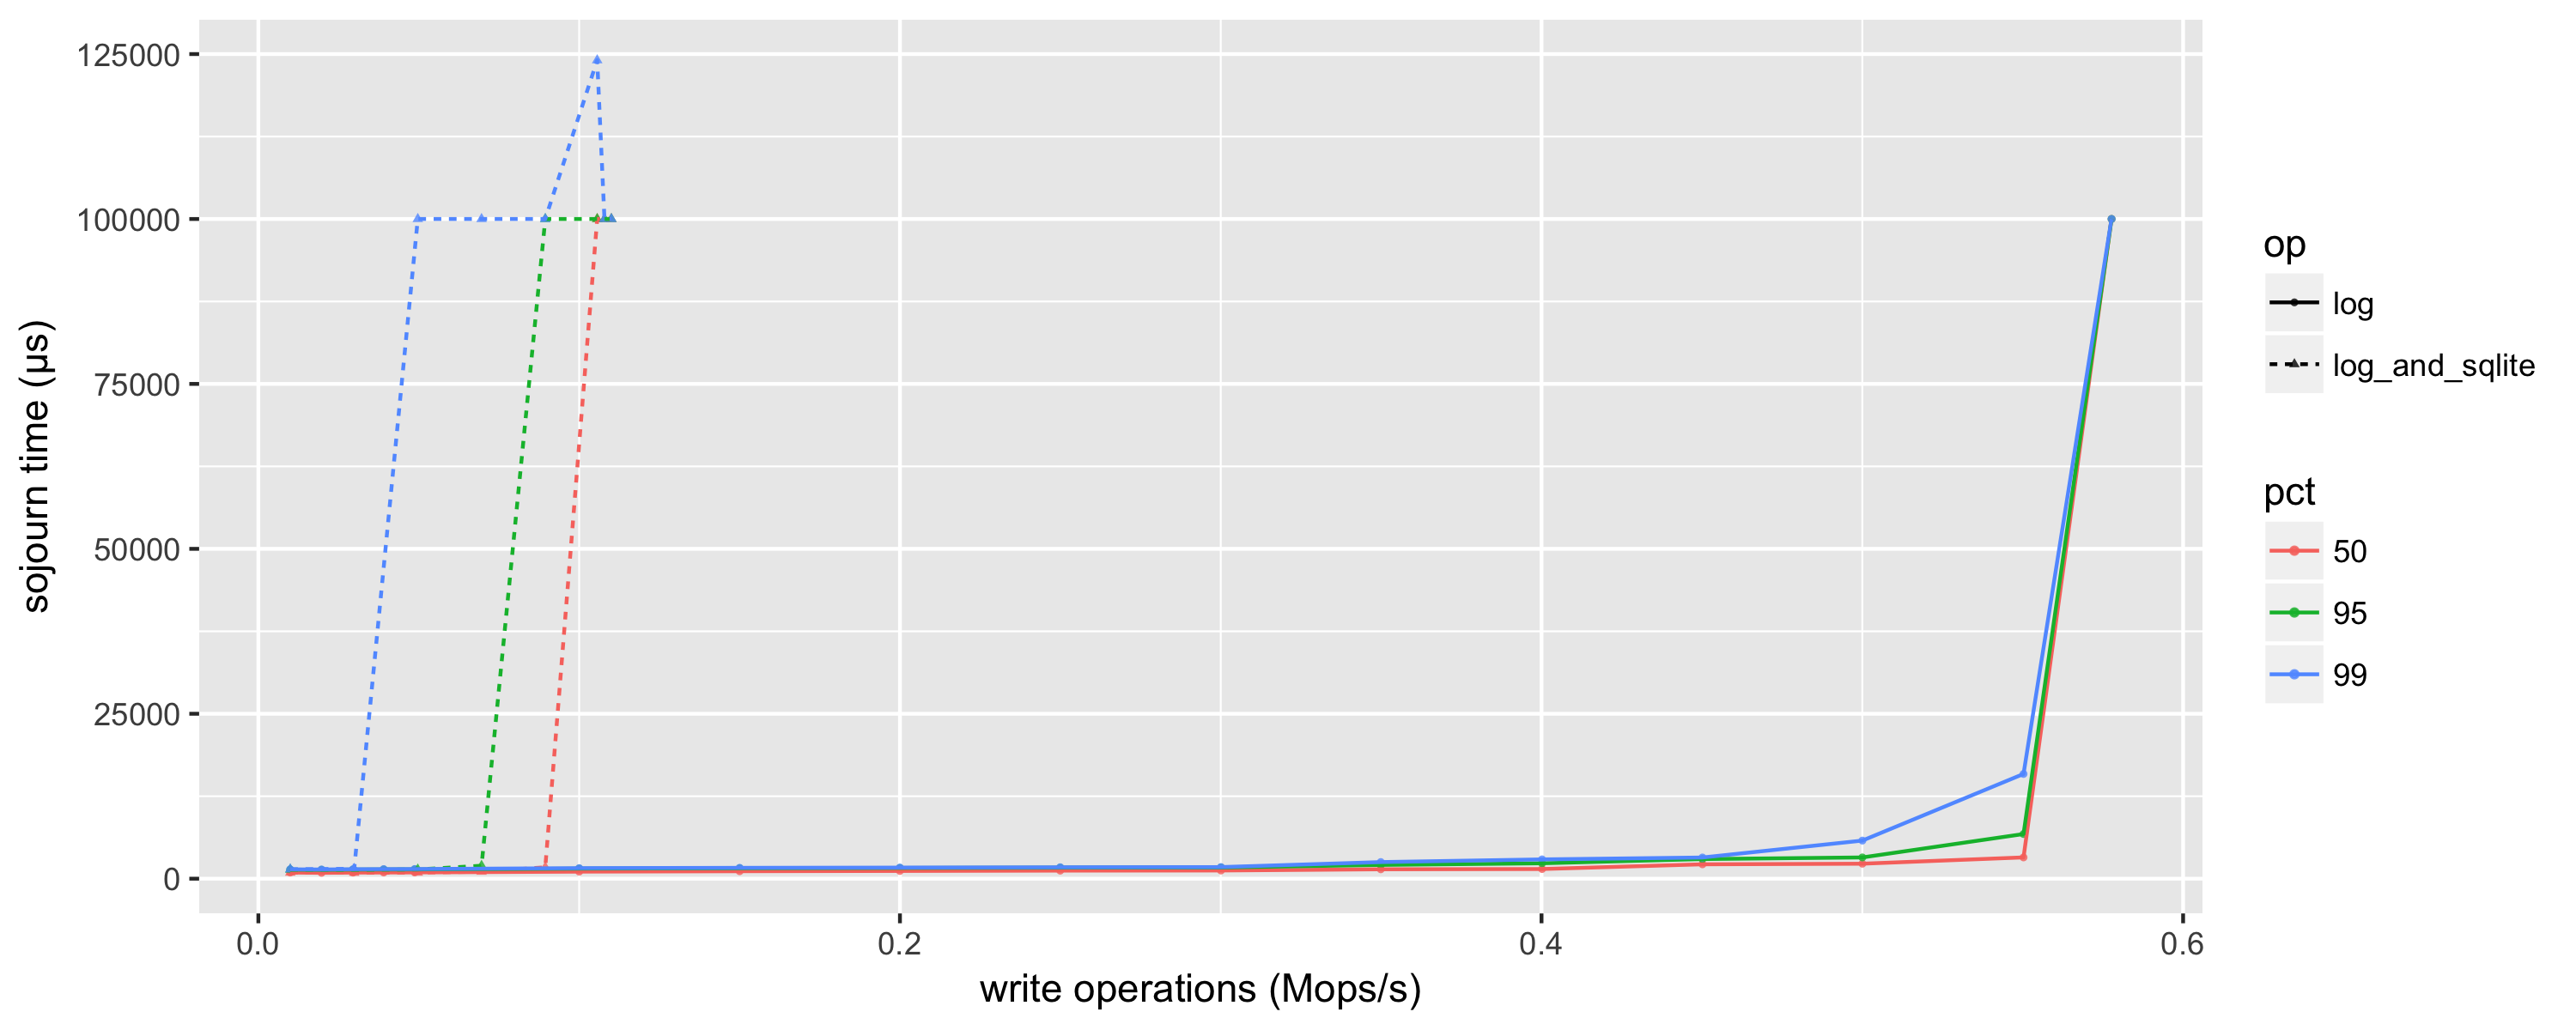
\includegraphics[width=\textwidth]{graphs/sqlite-soup-log}
  \caption{\
    Write-only throughput measured using the \code{vote} benchmark, comparing
    in-memory base nodes to persistent base nodes using SQLite---both examples
    use Soup's WAL for durability.
  }\label{graph:sqlite-soup-log}
\end{figure}

\todo{could write about the (failed) attempt of batching more writes together}

\subsubsection{Closing remarks}

The fact that SQLite works well out of the box without a lot of tuning is
definitely one of its strengths. Regardless, there are a few options that can be
tweaked, both ahead of compilation and at runtime. While disabling SQLite
features not needed for \code{PersistentState} and removing all mutex code had a
slight positive impact, the improvements were far from significant enough to
make a solid dent in the total throughput.

Maintaining SQLite indices---and thus randomly reading from and writing to
disk---on the main path is simply too slow. Does this imply that directly
maintaining B-tree on-disk index structures built specifically for Soup would
perform poorly as well? Possibly. While SQLite does have a lot of overhead
needed to support a wide range of features, and an even wider array of systems,
profiling clearly shows that the bulk of processing time is spent interacting
with durable storage as a result of B-tree maintenance.

\section{Persistent State with RocksDB}

How do we improve upon SQLite's low write throughput? One option would be to
only write to durable storage from background threads, avoiding the hit in
latency that comes with writing to and reading from disk. Instead, writes to
\code{PersistentState} could fill up an in-memory queue structure, which would
then later be flushed to persistent storage by background threads. Read
operations could then retrieve data from both the in-memory queue and the
slower---but persistent---SQLite. This might sound familiar, as it is
effectively a naive sketch of the log-structured merge-tree data structure
described in section~\ref{sec:rocksdb}, where writes are initially kept in an
in-memory buffer and later flushed to disk by background workers. That leaves us
with a good next step: embedding a storage engine that makes use of LSM-trees
internally, RocksDB.\@

While RocksDB and its LSM-trees should improve \code{PersistentState}'s write
throughput, it could at the same time introduce a further penalty to read
latency. This might not be too problematic though, as reads from
\code{PersistentState} should be more of a rare occurrence than writes: every
update Soup sees needs to be persisted to durable storage, whereas only a subset
of reads need to access \code{PersistentState} at all---most results should be
served by partial nodes further down the data-flow graph.

\subsection{Secondary Index Scheme}

Whereas SQLite includes support for a large subset of SQL features, RocksDB's
API is on a lower abstraction level. Limited to the functions necessary to
maintain a sorted key-value store, implementing support for secondary indices is
more of a challenge than with SQLite, where support for both primary and
secondary indices is built in. Building higher level abstractions on top of
key-value stores is becoming more and more common however, with plenty of
inspiration to be found in existing projects. Both CockroachDB~\cite{cockroach}
and MyRocks~\cite{myrocks} implement SQL-like functionality on top of RocksDB,
with sturdy indexing schemes at the core.

Prior to describing the final implementation, let us first iterate our way
towards a working index scheme. The next few sections describe separate,
working, implementations, where each step improves upon the last.

\subsubsection{Collection of rows}

Representing unique indices using a key-value store is fairly straight forward,
as each key maps to a single value. With secondary indices, this is no longer
the case, and a single key would need to represent multiple values. With
key-value stores where subsequent insertions are still retrievable with a single
read operation this would require no further abstractions. In RocksDB however,
each insertion effectively overwrites any existing values that might exist for
that key. So how do we emulate an API mapping a single key to multiple values
with the tools we have at hand? For a start, we could do exactly that, and store
multiple values in an array below each key. Insertions would then retrieve the
array of existing values, append the given value to that array, and write it
back to the same key---as shown in listing~\ref{lst:collection-secondary}.

\begin{listing}[H]
  \begin{minted}[frame=lines]{python}
Insert(key, value):
  # Retrieve and deserialize existing values:
  raw_values = Get(key)
  values = deserialize(raw_values) or []

  # Then, append our new value, serialize the collection and put it back:
  values += value
  Put(key, serialize(values))
  \end{minted}

  \caption{A naive secondary index implementation, where each key contains a
  collection of values.}\label{lst:collection-secondary}
\end{listing}

Unfortunately, this comes with the same write performance penalty as SQLite's
B-tree index structures: each write now has to first perform a random read
\textit{before} the new value can be written. This completely removes any
performance benefits we might gain from RocksDB's write-friendly LSM-tree
structure.

\subsubsection{Merge operator}

In addition to the more common \code{Get} and \code{Put} operations, RocksDB
supports an atomic read-modify-write operation through the \code{Merge}
method\footnote{\url{https://github.com/facebook/rocksdb/wiki/Merge-Operator}}.
This leads to the same result as in our previous implementation---with each key
mapping to a collection of values---without any random reads while writing.
Instead, RocksDB considers calls on the form \code{Merge(key, value)} as an
\textit{intent} to merge the values, and persists it as such. These intents can
then be processed later, during background compactions (see
section~\ref{sec:compactions}) and read operations.

\begin{listing}[H]
  \begin{minted}[frame=lines]{python}
MergeOperator(key, existing, operations):
  # Retrieve and deserialize existing values:
  raw_values = Get(key)
  values = deserialize(raw_values) or []

  # Then, append all Merge(key, value) operations:
  for op in operations
    values += deserialize(op)

  # Finally, serialize and return the new list:
  serialize(values)
  \end{minted}

  \caption{A RocksDB merge operator, appending any given values to an array.}\label{lst:merge-fn}
\end{listing}

This moves some of the work from writing to reading, as a read operation now has
to find all merge operands and process them before returning. Unfortunately,
this also introduces an unnecessary amount of serialization. RocksDB does not
know how to deal with anything but byte streams, and so both the input and
output to the merge operator has to be serialized, regardless of the fact that
the final result will have to be deserialized again when read by the caller.
This could potentially be improved through a smarter serialization scheme, where
values could be appended to the serialized array without deserialization, but
let us first consider an alternative without the merge operator altogether.

\subsubsection{Iteration}

Up until now we have considered options where each index value takes up a single
key, through various methods of making the value portion of a key-value pair
plural. Instead, we will now modify the key slightly to achieve uniqueness,
while still retaining the ability to retrieve its corresponding value from the
original key. The latter is possible through \textit{iteration}. By making sure
keys that refer to the same index value are placed next to each other we can
find the first key, and then iterate forward until we reach a separate index
value. That way, each key only needs to point to a single value, while
subsequent insertions can function without needing to retrieve any existing
values.

How do we ensure that multiple keys are placed next to each other, while still
remaining unique? One way of doing so would be with a monotonically increasing
sequence number appended to the end of each key, incremented on subsequent
insertions.

% TODO:
% The examples will use the same table, containing three columns and two indices:
% \code{(id, name, country)}, with a primary index on \code{id} and a secondary
% index on \code{(country)}.
